\definecolor{plot_orange}{rgb}{1, 0.639, 0}
\definecolor{plot_red}{rgb}{0.973, 0.463, 0.427}
\definecolor{plot_blue}{rgb}{0.153, 0.682, 0.937}
\definecolor{plot_green}{rgb}{0, 0.729, 0.22}
\definecolor{plot_gray}{rgb}{0.4, 0.4, 0.4}

In this chapter, we compare five different methods: Sparse, our SQL Einsum implementation, Torch, our 
Sparse Einsum, and our Legacy Sparse Einsum across various problems. In the plots, we will mark
our implementations, SQL Einsum, Sparse Einsum and Legacy Sparse Einsum with an asterisk (*). In the
first experiment, we evaluate their performance on three real-world instances of the
``Einsum Benchmark"~\cite{einsum_benchmark} dataset, which consists of real problems with complex
tensor computations. In the second experiment, we asses their performance on various random tensor
hypernetworks. For all computations, every method receives the same contraction path, which is computed
via cgreedy 0.0.3 before measuring the methods performance. It should be noted that we use Torch 2.0.1+cu118 as well
as Sparse 0.15.4 as backends for opt\_einsum 3.3.0. This allows us to compute Einsum expressions with UTF-8 characters using Torch and Sparse. The SQL queries to evaluate the Einsum problems
are computed using the Python module sqlite3 2.6.0, which uses SQLite 3.38.4 as the database engine.
The experiments are performed on a machine with an Intel i5-9600K 6-core processor running Windows 11
Pro with 16 GB of RAM. Each core has a base frequency of 3.7 GHz and a max boost frequency of 4.6 GHz.
To compile the algorithm, we use MSVC 14.34.31931. The evaluation is done in Python 3.11.0.

\section{Einsum Benchmark Instances}
In this section, we discuss the results of the methods on three real model counting problems.
We chose these instances because they lead to sparse intermediate tensors and they are small enough
to fit into memory on the machine we are benchmarking on. For each instance, Table \ref{tab:instance:data}
lists the name, the number of input tensors, and the average density of the tensors after optimizing
the contraction path for size.
\begin{table}[hbp]
    \caption{Instance Data with Tensor Count and Average Density.}
    \label{tab:instance:data}
    \centering
    \begin{tabularx}{0.8\textwidth}{l  >{\raggedleft\arraybackslash}X  >{\raggedleft\arraybackslash}X}
        \toprule
        \textbf{Instance} & \textbf{Tensors} & \textbf{Average Density} \\
        \midrule
        mc\_2021\_027     & 331              & 0.021689                 \\
        mc\_2021\_036     & 9553             & 0.000545                 \\
        mc\_2022\_087     & 7345             & 0.001138                 \\
        \bottomrule
    \end{tabularx}
\end{table}
\\
Figure \ref{fig:exp:instances} shows each method's iterations per second (it/s) on a logarithmic scale,
highlighting the disparities in performance. Our two implementations, Sparse Einsum and Legacy Sparse
Einsum, show consistently strong performance on the first instance, mc\_2021\_027, with Sparse Einsum
achieving the highest it/s, closely followed by Legacy Sparse Einsum. As we move to the more challenging
second instance, mc\_2021\_036, Sparse Einsum and Legacy Sparse Einsum perform the best out of all methods,
with Sparse and SQL not being able to compute the result due to a limit for the number of dimensions
for Sparse and SQL running out of memory. Torch is much slower than our methods. On the final instance,
mc\_2022\_087, Sparse Einsum and Legacy Sparse Einsum continue to outperform the other methods. SQL is
again, not capable of finishing the computation. Compared to the others, Sparse shows the lowest it/s.

\begin{figure}[H]
    \centering
    \begin{tikzpicture}
        \begin{axis}[
                ybar, axis on top,
                height=8cm, width=12cm,
                bar width=0.4cm,
                ymajorgrids, tick align=inside,
                enlarge y limits={value=.1,upper},
                enlarge x limits=0.3, % Reduce this value to bring the groups closer
                ymode=log, % Use logarithmic scale for the y-axis
                log origin=infty, % Start the log scale at the smallest positive value
                ymin=1e-3, ymax=12, % Adjust the minimum and maximum y-axis values
                axis x line*=bottom,
                axis y line*=left,
                y axis line style={opacity=0},
                tickwidth=0pt,
                legend style={
                        at={(0.5,1.05)}, % Position above the plot
                        anchor=south, % Anchor to the south of the legend
                        legend columns=3, % Arrange entries side by side
                        column sep=1ex, % Space between columns
                        draw=none, % Remove the border
                        fill=none, % Remove the background fill
                        legend cell align=left
                    },
                legend image code/.code={
                        \draw [#1] (0cm,-0.1cm) rectangle (0.28cm,0.25cm); },
                ylabel={Iterations per Second (it/s)},
                symbolic x coords={
                        mc\_2021\_027, mc\_2021\_036, mc\_2022\_087},
                xtick=data,
            ]
            \addplot [draw=none, fill=plot_blue] coordinates {
                    (mc\_2021\_027, 0.613)
                    (mc\_2021\_036, 0.00001)
                    (mc\_2022\_087, 0.005)};
            \addplot [
                draw=none,
                fill=plot_green,
                postaction={
                        pattern=crosshatch,
                        pattern color=plot_green!30
                    }
            ] coordinates {
                    (mc\_2021\_027, 0.632)
                    (mc\_2021\_036, 0.00001)
                    (mc\_2022\_087, 0.000)};
            \addplot [
                draw=none,
                fill=plot_red,
                postaction={
                        pattern=grid,
                        pattern color=plot_red!30
                    }
            ] coordinates {
                    (mc\_2021\_027, 3.258)
                    (mc\_2021\_036, 0.009)
                    (mc\_2022\_087, 0.056)};
            \addplot [
                draw=none,
                fill=plot_gray,
                postaction={
                        pattern=horizontal lines,
                        pattern color=plot_gray!30
                    }
            ] coordinates {
                    (mc\_2021\_027, 7.339)
                    (mc\_2021\_036, 0.056)
                    (mc\_2022\_087, 0.154)};
            \addplot [
                draw=none,
                fill=plot_orange,
                postaction={
                        pattern=vertical lines,
                        pattern color=plot_gray
                    }
            ] coordinates {
                    (mc\_2021\_027, 10.052)
                    (mc\_2021\_036, 0.074)
                    (mc\_2022\_087, 0.167)};

            \legend{Sparse, SQL Einsum*, Torch, Legacy Sparse Einsum*, Sparse Einsum*}
        \end{axis}
    \end{tikzpicture}
    \caption{Performance comparison of different methods for multiple instances 
    on a logarithmic scale.}
    \label{fig:exp:instances}
\end{figure}

\section{Random Tensor Hypernetworks}
To evaluate the performance of our implementations across a variety of properties that Einsum
problems may exhibit, we generate Einsum expressions representing random tensor hypernetworks
\cite{einsum_benchmark}, with each experiment featuring a single varying parameter. For every new
parameter the results are evaluated using ten differently seeded random tensor hypernetworks
generated with identical parameters. We then evaluate each methods performance on the problem
ten times to get an average it/s. To generate the random tensor hypernetworks, we use the following
parameters as a basis, varying one for each experiment:
\begin{description}[leftmargin=!,labelwidth=\widthof{\textbf{single\_summation\_indices = 15:}}]
    \item [number\_of\_tensors = 6:] Specifies the total number of tensors in the hypernetwork.

    \item [regularity = 3.0:] Defines the regularity of the tensor network, which influences how many
          indices/axes each tensor shares on average.

    \item [max\_tensor\_order = 15:] Sets the maximum order (number of axes/dimensions) of the tensors.

    \item [max\_edge\_order = 3:] Determines the maximum order of hyperedges in the tensor network.

    \item [output\_indices = 0:] Specifies the number of output indices or axes
          (i.e., non-contracted indices).

    \item [single\_summation\_indices = 15:] Indicates the number of indices that are not connected to
          any other tensors and do not appear in the output.

    \item [min\_axis\_size = 2:] Sets the minimum size of an axis/index (dimension) of the tensors.

    \item [max\_axis\_size = 15:] Sets the maximum size of an axis/index (dimension) of the tensors.

    \item [density = 0.001:] Indicates how many elements are non-zero compared to the total number of
          elements in the tensor.
\end{description}
\noindent
First, we generate problems where we vary the maximum size of dimensions (max\_ax-is\_size)
from 2 to 15. Figure \ref{fig:exp:max_dim_size} shows the performance for the different
dimension sizes. The performance of all methods naturally decreases when the size of dimensions
grows. However, the rate of this degradation differs significantly between the methods.
Sparse performance decreases quickly when the maximum number of dimensions that the tensors
can have increases. It starts of with around the same it/s as SQL but declines faster than
the other methods, coming in last with about the same performance as Torch. In general,
SQL Einsum is superior for small till medium sizes of dimensions, but it also declines more
steeply in comparison to all other methods. The SQL implementations iterations per second rise,
when the maximum size of dimensions increases from two to six and from thereon decreases constantly.
Sparse Einsum and the legacy version of Sparse Einsum demonstrated very similar trends,
though the legacy variant performed worse at all dimension sizes than the newer implementation.
Still, both surpass the other methods with rising size of dimensions.

\begin{figure}[H]
    \centering
    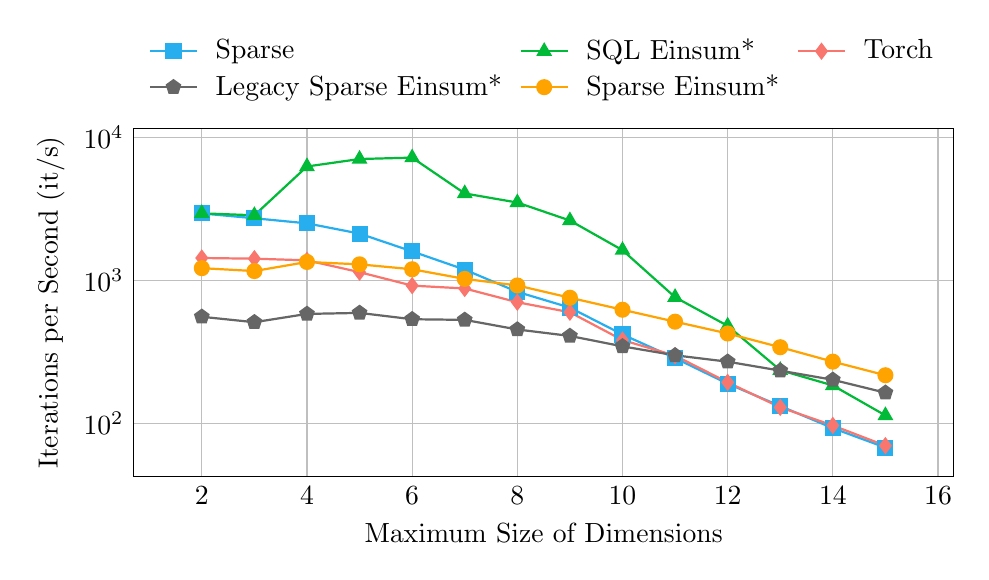
\begin{tikzpicture}
        \begin{semilogyaxis}[
                xlabel={Maximum Size of Dimensions},
                ylabel={Iterations per Second (it/s)},
                grid=major,
                mark size=2.5pt,
                width=12cm,
                height=6cm,
                enlargelimits=0.1,
                xtick style={draw=none},  % Remove x-axis tick marks
                ytick style={draw=none},  % Remove y-axis tick marks
                log basis y=10,           % Set base 10 for y-axis
                legend style={
                        at={(0.5,1.05)}, % Position above the plot
                        anchor=south, % Anchor to the south of the legend
                        legend columns=3, % Arrange entries side by side
                        column sep=1ex, % Space between columns
                        draw=none, % Remove the border
                        fill=none, % Remove the background fill
                        legend cell align=left
                    }
            ]

            % Sparse_Time (Square marker)
            \addplot[
                color=plot_blue,
                mark=square*,
                thick
            ] coordinates {
                    (2, 2949.141) (3, 2728.197) (4, 2514.223) (5, 2130.835)
                    (6, 1600.128) (7, 1193.220) (8, 833.779) (9, 647.050)
                    (10, 419.688) (11, 286.894) (12, 190.042) (13, 132.532)
                    (14, 92.850) (15, 67.926)
                };
            \addlegendentry{Sparse}

            % SQL_Einsum_Time (Triangle marker)
            \addplot[
                color=plot_green,
                mark=triangle*,
                thick
            ] coordinates {
                    (2, 2954.971) (3, 2861.648) (4, 6282.668) (5, 7085.857)
                    (6, 7246.113) (7, 4068.557) (8, 3514.551) (9, 2631.675)
                    (10, 1632.327) (11, 765.026) (12, 482.367) (13, 236.127)
                    (14, 184.713) (15, 113.928)
                };
            \addlegendentry{SQL Einsum*}

            % Torch_Time (Diamond marker)
            \addplot[
                color=plot_red,
                mark=diamond*,
                thick
            ] coordinates {
                    (2, 1438.503) (3, 1422.954) (4, 1385.463) (5, 1145.090)
                    (6, 921.999) (7, 880.472) (8, 705.581) (9, 600.319)
                    (10, 383.697) (11, 298.314) (12, 194.233) (13, 129.782)
                    (14, 96.937) (15, 69.999)
                };
            \addlegendentry{Torch}

            % Legacy_Sparse_Einsum_Time (Pentagon marker)
            \addplot[
                color=plot_gray,
                mark=pentagon*,
                thick
            ] coordinates {
                    (2, 558.216) (3, 511.409) (4, 584.589) (5, 594.116)
                    (6, 536.521) (7, 531.115) (8, 454.884) (9, 409.967)
                    (10, 346.686) (11, 300.110) (12, 270.774) (13, 234.450)
                    (14, 202.283) (15, 164.314)
                };
            \addlegendentry{Legacy Sparse Einsum*}

            % Sparse_Einsum_Time (Circle marker)
            \addplot[
                color=plot_orange,
                mark=*,
                thick
            ] coordinates {
                    (2, 1221.739) (3, 1165.713) (4, 1349.421) (5, 1298.878)
                    (6, 1199.998) (7, 1027.373) (8, 924.336) (9, 758.730)
                    (10, 625.246) (11, 515.746) (12, 426.570) (13, 341.911)
                    (14, 270.924) (15, 217.710)
                };
            \addlegendentry{Sparse Einsum*}

        \end{semilogyaxis}
    \end{tikzpicture}
    \caption{Performance of different methods as a function of maximum dimension size on a logarithmic scale.
        The plot shows the number of iterations per second for each method.}
    \label{fig:exp:max_dim_size}
\end{figure}

\noindent
The results illustrated in Figure \ref{fig:exp:max_num_dim} show how the computational performance
of each method varies with increasing dimensionality (max\_tensor\_order) in tensor hypernetworks.
All of the methods it/s decline as dimensionality increases. SQL Einsum starts off with the
best performance, but declines rapidly, getting surpassed by our Sparse Einsum and our Legacy Sparse
Einsum as well as Sparse. Torch's performance starts of slightly higher than Legacy Sparse Einsum's,
but quickly recedes with the growing number of dimensions. Overall, Sparse Einsum and Legacy Sparse
Einsum handle the increasing dimensionality best, with Sparse Einsum displaying the highest iterations
per second for problems with higher dimensionality.

\begin{figure}[H]
    \centering
    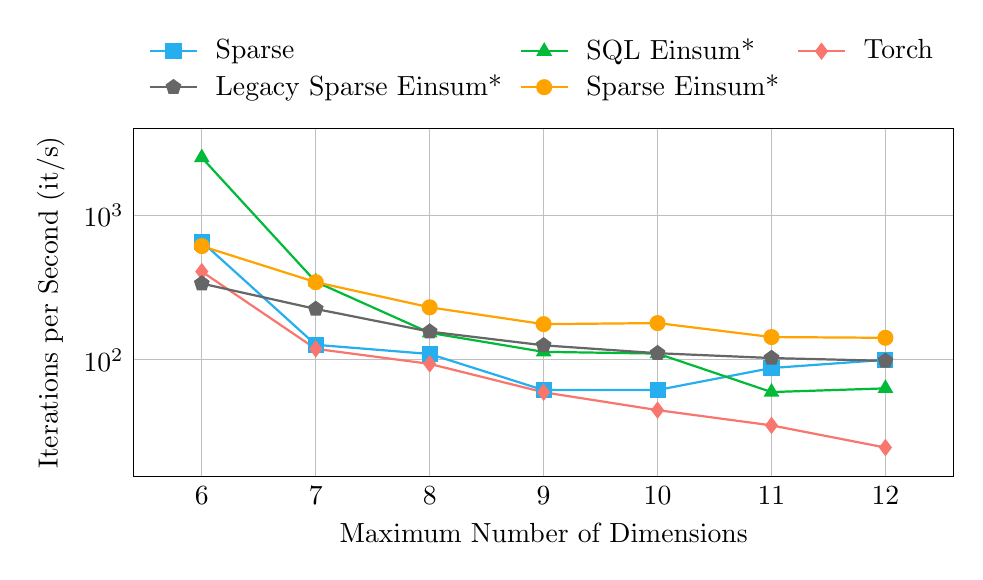
\begin{tikzpicture}
        \begin{axis}[
                xlabel={Maximum Number of Dimensions},
                ylabel={Iterations per Second (it/s)},
                grid=major,
                mark size=2.5pt,
                width=12cm,
                height=6cm,
                enlargelimits=0.1,
                xtick style={draw=none},
                ytick style={draw=none},
                ymode=log,
                log basis y=10,           % Set base 10 for y-axis
                legend style={
                        at={(0.5,1.05)},
                        anchor=south,
                        legend columns=3,
                        column sep=1ex,
                        draw=none,
                        fill=none,
                        legend cell align=left
                    }
            ]

            % Sparse_Time (Square marker)
            \addplot[
                color=plot_blue,
                mark=square*,
                thick
            ] coordinates {
                    (6, 656.079) (7, 127.233) (8, 109.917) (9, 61.866)
                    (10, 61.965) (11, 87.939) (12, 100.175)
                };
            \addlegendentry{Sparse}

            % SQL_Einsum_Time (Triangle marker)
            \addplot[
                color=plot_green,
                mark=triangle*,
                thick
            ] coordinates {
                    (6, 2500.888) (7, 346.885) (8, 153.930) (9, 113.701)
                    (10, 110.663) (11, 59.971) (12, 63.598)
                };
            \addlegendentry{SQL Einsum*}

            % Torch_Time (Diamond marker)
            \addplot[
                color=plot_red,
                mark=diamond*,
                thick
            ] coordinates {
                    (6, 407.781) (7, 119.323) (8, 93.899) (9, 59.792)
                    (10, 44.990) (11, 35.300) (12, 24.798)
                };
            \addlegendentry{Torch}

            % Legacy_Sparse_Einsum_Time (Pentagon marker)
            \addplot[
                color=plot_gray,
                mark=pentagon*,
                thick
            ] coordinates {
                    (6, 337.235) (7, 225.109) (8, 156.957) (9, 126.146)
                    (10, 111.298) (11, 103.061) (12, 98.580)
                };
            \addlegendentry{Legacy Sparse Einsum*}

            % Sparse_Einsum_Time (Circle marker)
            \addplot[
                color=plot_orange,
                mark=*,
                thick
            ] coordinates {
                    (6, 611.765) (7, 344.672) (8, 231.014) (9, 176.694)
                    (10, 179.796) (11, 143.914) (12, 142.225)
                };
            \addlegendentry{Sparse Einsum*}

        \end{axis}
    \end{tikzpicture}
    \caption{Performance of different methods as a function of the maximum number of dimensions on a logarithmic scale.
        The plot shows the number of iterations per second for each method.}
    \label{fig:exp:max_num_dim}
\end{figure}

\noindent
Figure \ref{fig:exp:num_tensors} shows each method's performance with increasing number of tensors
(number\_of\_tensors). We set max\_tensor\_order and max\_axis\_size to nine,
to be able to fit the generated tensors into memory. Sparse displays a decent performance to start with but
drops off significantly as tensor count increases, being by far the slowest method for larger numbers of
tensors. SQL Einsum starts off strongly, and while it gets slower with the rising number of tensors, it
still outperforms the other methods. Torch is rather stable but decreasing and remains more efficient than
Sparse at higher tensor counts. Sparse Einsum and Legacy Sparse Einsum decline in nearly identical
fashion, with Sparse Einsum constantly performing better than Legacy Sparse Einsum. Legacy Sparse Einsum
manages to outperform Torch in iterations per second with larger numbers of tensors.

\begin{figure}[H]
    \centering
    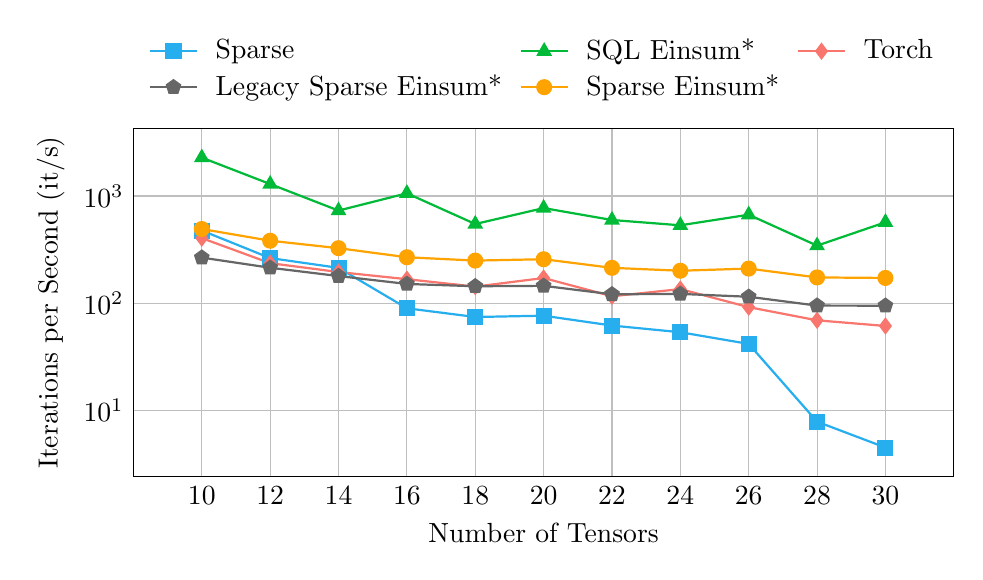
\begin{tikzpicture}
        \begin{semilogyaxis}[
                xlabel={Number of Tensors},
                ylabel={Iterations per Second (it/s)},
                grid=major,
                mark size=2.5pt,
                width=12cm,
                height=6cm,
                enlargelimits=0.1,
                xtick style={draw=none},
                ytick style={draw=none},
                xtick={10, 12, 14, 16, 18, 20, 22, 24, 26, 28, 30}, % Correct x-ticks
                xticklabels={10, 12, 14, 16, 18, 20, 22, 24, 26, 28, 30}, % Correct labels for x-ticks
                legend style={
                        at={(0.5,1.05)}, % Position above the plot
                        anchor=south, % Anchor to the south of the legend
                        legend columns=3, % Arrange entries side by side
                        column sep=1ex, % Space between columns
                        draw=none, % Remove the border
                        fill=none, % Remove the background fill
                        legend cell align=left
                    }
            ]

            % Sparse_Time (Square marker)
            \addplot[
                color=plot_blue,
                mark=square*,
                thick
            ] coordinates {
                    (10, 476.545) (12, 263.609) (14, 213.613) (16, 89.564)
                    (18, 74.276) (20, 76.383) (22, 61.785) (24, 53.520)
                    (26, 41.633) (28, 7.829) (30, 4.485)
                };
            \addlegendentry{Sparse}

            % SQL_Time (Triangle marker)
            \addplot[
                color=plot_green,
                mark=triangle*,
                thick
            ] coordinates {
                    (10, 2284.108) (12, 1294.497) (14, 731.881) (16, 1061.477)
                    (18, 548.178) (20, 772.391) (22, 597.661) (24, 533.237)
                    (26, 669.754) (28, 344.313) (30, 569.061)
                };
            \addlegendentry{SQL Einsum*}

            % Torch_Time (Diamond marker)
            \addplot[
                color=plot_red,
                mark=diamond*,
                thick
            ] coordinates {
                    (10, 404.718) (12, 236.199) (14, 195.213) (16, 167.394)
                    (18, 142.753) (20, 171.697) (22, 116.004) (24, 135.279)
                    (26, 91.784) (28, 69.143) (30, 61.248)
                };
            \addlegendentry{Torch}

            % Legacy_Sparse_Einsum_Time (Pentagon marker)
            \addplot[
                color=plot_gray,
                mark=pentagon*,
                thick
            ] coordinates {
                    (10, 266.300) (12, 214.103) (14, 179.091) (16, 151.105)
                    (18, 143.827) (20, 145.156) (22, 120.983) (24, 122.016)
                    (26, 114.738) (28, 94.909) (30, 94.717)
                };
            \addlegendentry{Legacy Sparse Einsum*}

            % Sparse_Einsum_Time (Circle marker)
            \addplot[
                color=plot_orange,
                mark=*,
                thick
            ] coordinates {
                    (10, 492.369) (12, 382.741) (14, 326.109) (16, 268.279)
                    (18, 249.704) (20, 257.161) (22, 213.647) (24, 200.779)
                    (26, 210.283) (28, 173.847) (30, 171.929)
                };
            \addlegendentry{Sparse Einsum*}

        \end{semilogyaxis}
    \end{tikzpicture}
    \caption{Performance of different methods as a function of the number of tensors on a logarithmic scale. We set
        \mbox{max\_tensor\_order = max\_axis\_size = 9}, because for larger values the tensors may not
        fit into memory upon generation.}
    \label{fig:exp:num_tensors}
\end{figure}

\noindent
Figure \ref{fig:exp:density} shows the performance trends of the different methods with
decreasing density (density). We decrease the density of the same tensor hypernetworks for each step.
Some methods improve drastically as the density decreases, while others remain about the same. In
particular, SQL Einsum shows a dramatic improvement with lower densities, quickly accelerating from low
performance at high densities to exceptional performance at the sparsest levels, generating an
S-curve. Sparse Einsum Legacy and Sparse Einsum both exhibit strong performance improvements as
density decreases. That being said, Sparse Einsum tends to perform better than its legacy Sparse
Einsum variant, especially at lower densities. On the other hand, Torch is quite stable
across different densities, only showing minor fluctuations as the density decreases. The same can
also be said for Sparse, which shows very little change across the density spectrum. The contrast
emphasizes that some methods perform much better on dense data, while others are specialized
for sparse data; the efficiency gains grow more dramatic as the data gets sparser.

\begin{figure}[H]
    \centering
    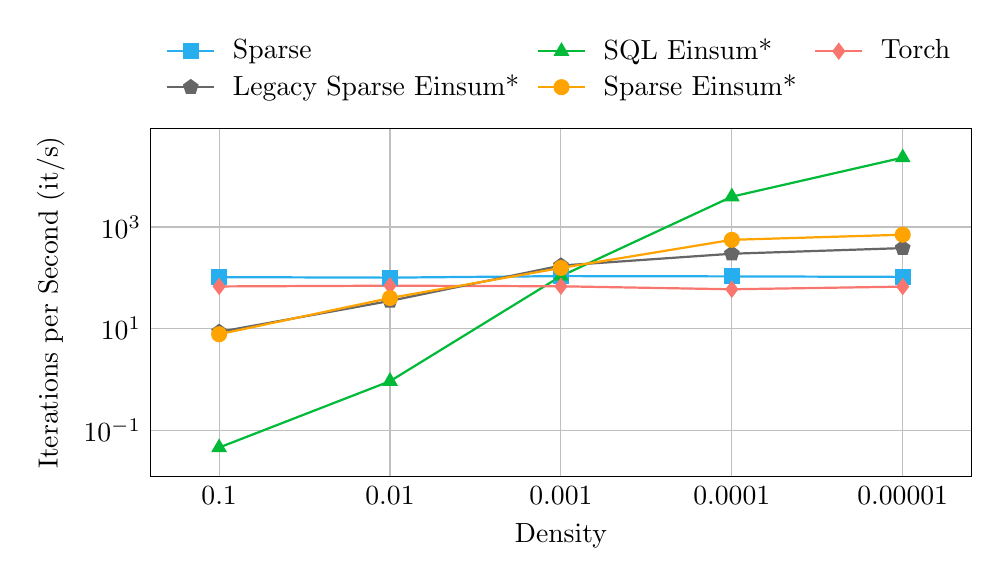
\begin{tikzpicture}
        \begin{semilogyaxis}[
                xlabel={Density},
                ylabel={Iterations per Second (it/s)},
                grid=major,
                mark size=2.5pt,
                width=12cm,
                height=6cm,
                enlargelimits=0.1,
                xtick style={draw=none},  % Remove x-axis tick marks
                ytick style={draw=none},  % Remove y-axis tick marks
                xtick={0.1, 0.01, 0.001, 0.0001, 0.00001}, % Specify custom x-axis ticks
                xticklabels={0.1, 0.01, 0.001, 0.0001, 0.00001}, % Set custom labels
                xmode=log,                % Logarithmic scale for x-axis
                log basis x=10,           % Set base 10 for x-axis
                x dir=reverse,
                legend style={
                        at={(0.5,1.05)}, % Position above the plot
                        anchor=south, % Anchor to the south of the legend
                        legend columns=3, % Arrange entries side by side
                        column sep=1ex, % Space between columns
                        draw=none, % Remove the border
                        fill=none, % Remove the background fill
                        legend cell align=left
                    }
            ]

            \addplot[
                color=plot_blue,
                mark=square*,
                thick
            ] coordinates {
                    (0.1, 103.350) (0.01, 101.109) (0.001, 108.362)
                    (0.0001, 106.939) (0.00001, 104.600)
                };
            \addlegendentry{Sparse}

            \addplot[
                color=plot_green,
                mark=triangle*,
                thick
            ] coordinates {
                    (0.1, 0.046) (0.01, 0.929) (0.001, 108.230)
                    (0.0001, 3952.256) (0.00001, 23169.600)
                };
            \addlegendentry{SQL Einsum*}

            \addplot[
                color=plot_red,
                mark=diamond*,
                thick
            ] coordinates {
                    (0.1, 67.884) (0.01, 70.186) (0.001, 68.328)
                    (0.0001, 59.668) (0.00001, 67.295)
                };
            \addlegendentry{Torch}

            \addplot[
                color=plot_gray,
                mark=pentagon*,
                thick
            ] coordinates {
                    (0.1, 8.646) (0.01, 35.231) (0.001, 174.506)
                    (0.0001, 298.441) (0.00001, 385.398)
                };
            \addlegendentry{Legacy Sparse Einsum*}

            \addplot[
                color=plot_orange,
                mark=*,
                thick
            ] coordinates {
                    (0.1, 7.789) (0.01, 40.1406) (0.001, 156.571)
                    (0.0001, 560.104) (0.00001, 706.623)
                };
            \addlegendentry{Sparse Einsum*}

        \end{semilogyaxis}
    \end{tikzpicture}
    \caption{Performance comparison of different methods for varying densities on a logarithmic scale.
    The plot shows the iterations per second for each method.}
    \label{fig:exp:density}
\end{figure}